\chapter{Jitter}
\label{Jitter}
\section{Notizen}
    
\section{Überblick}
\begin{itemize}
	\item Stundenwiederholung
	\item Überblick über Software Pakete
	\item Vizzie
	\item kommunikation pd/max?
	\item Aufgabe: Video Laden, Abspielen, Audio analyse, modulation eines Effektes, Recording.
	\item Jitter Matrix (Wiederholung?)
	\item Audio analogien: jit.convolve, anti-aliasing(Open GL), jit.charmap(lookup table)

	\item Open GL, anti aliasing, 
\end{itemize}

\section{Andere Software Pakete für visuelle Echtzeit Arbeit}
Graphik Programmierumgebungen
\begin{itemize}
	\item Jitter
	\item Gem (pure Data)
	\item vvvv
	\item TouchDesigner
	\item processing
	\item Quarz Composer
\end{itemize}
\glqq{}Professionelle\grqq{} weniger offene Systeme(weniger programmier-orientiert)
\begin{itemize}
	\item Watchout
	\item Vizrt
	\item Ventuz
\end{itemize}
Game Engines
\begin{itemize}
	\item Unreal 4
	\item Unity
	\item Cry Enigine
	\item ...
\end{itemize}


\section{Introduction}

\begin{figure}[h]
	\begin{center}
		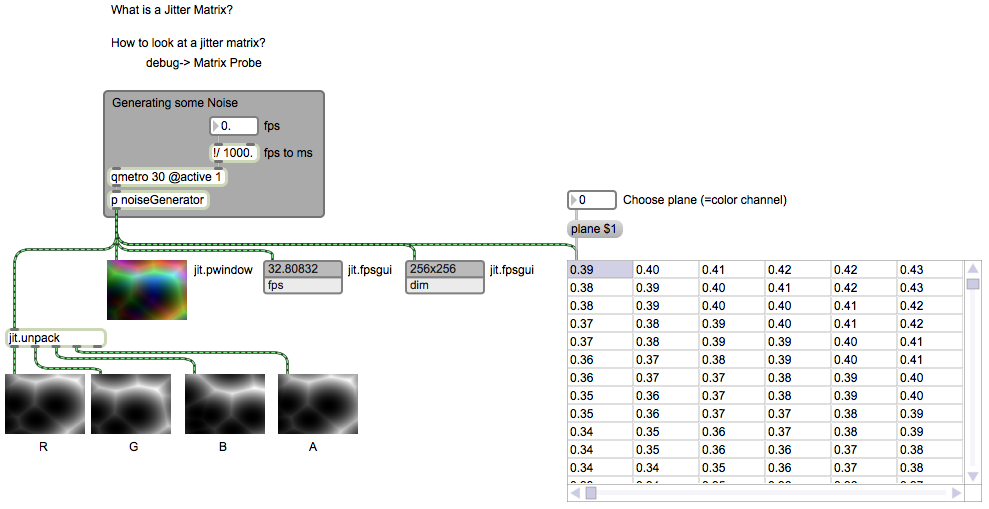
\includegraphics[width = 14cm]{img/lookAtMatrix.png}
		\caption{How to look at a jitter matrix}
		\label{fig:howToLook}
	\end{center}
\end{figure}

\begin{figure}[h]
	\begin{center}
		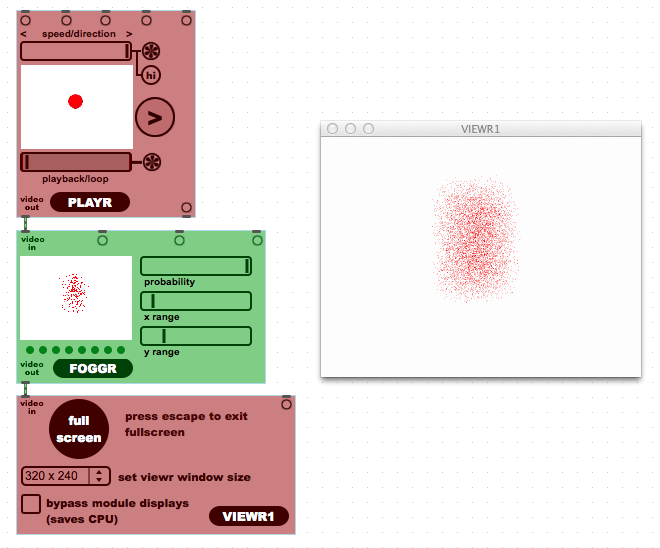
\includegraphics[width = 14cm]{img/hiLevelJitter.png}
		\caption{hi Level Jitter}
		\label{fig:hiLevelJitter}
	\end{center}
\end{figure}

\begin{figure}[h]
	\begin{center}
		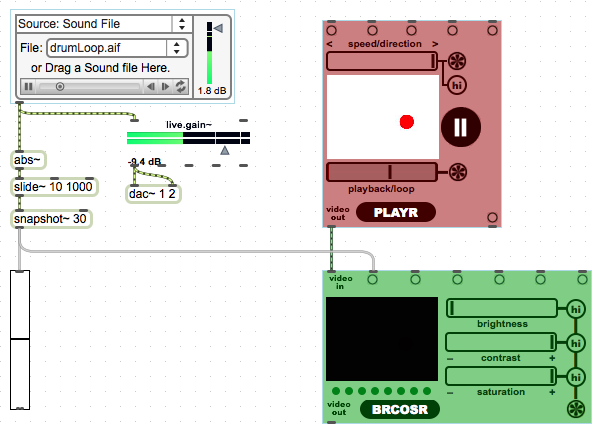
\includegraphics[width = 14cm]{img/VizzieAudioModulated.png}
		\caption{VizzieAudioModulated}
		\label{fig:VizzieAudioModulated}
	\end{center}
\end{figure}

\begin{figure}[h]
	\begin{center}
		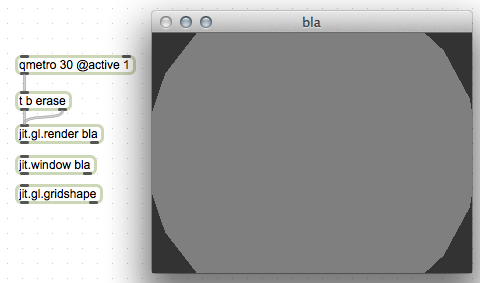
\includegraphics[width = 14cm]{img/basicGL.png}
		\caption{basicGL}
		\label{fig:basicGL}
	\end{center}
\end{figure}


\begin{figure}[h]
	\begin{center}
		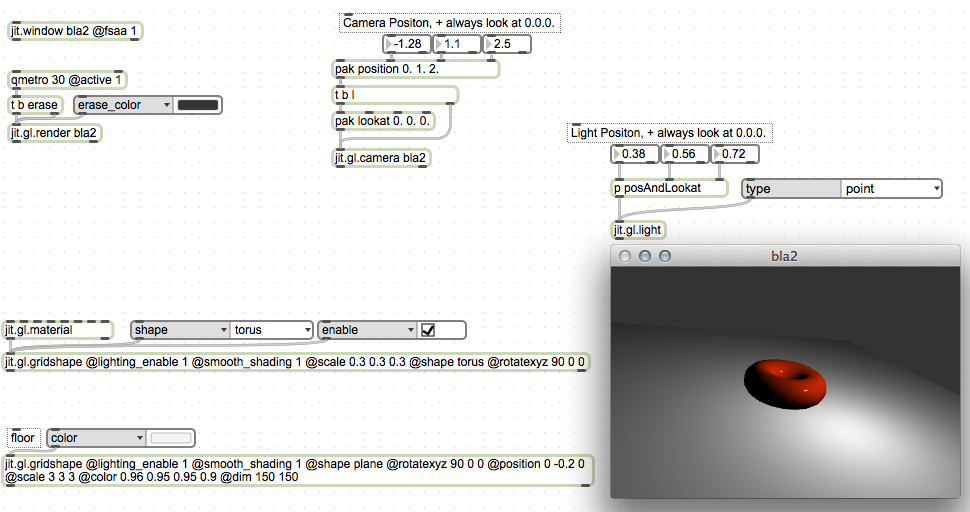
\includegraphics[width = 14cm]{img/openGLAdvanced.png}
		\caption{openGLAdvanced}
		\label{fig:openGLAdvanced}
	\end{center}
\end{figure}


\begin{figure}[h]
	\begin{center}
		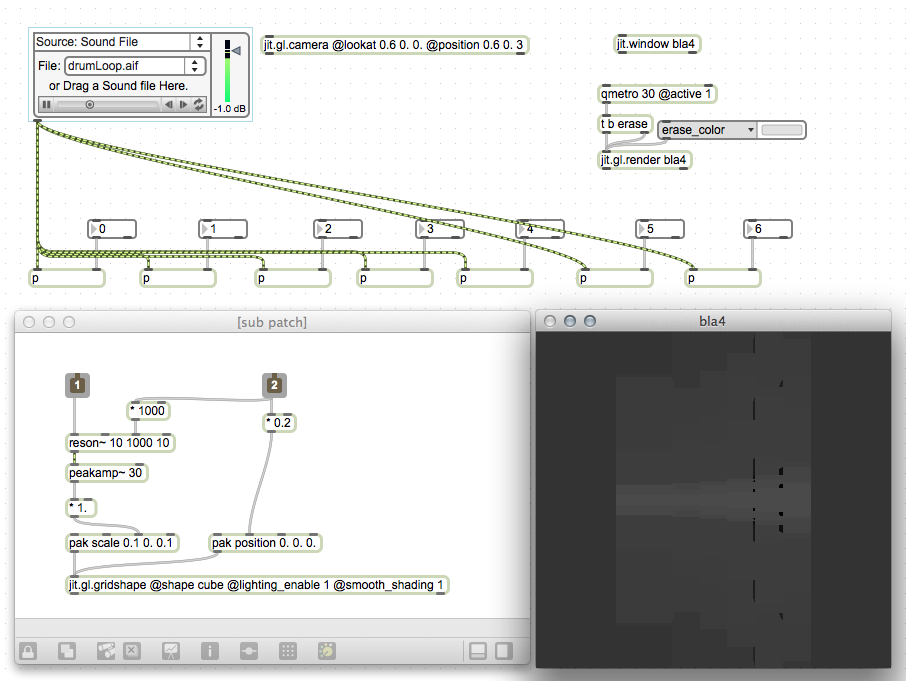
\includegraphics[width = 14cm]{img/specViz.png}
		\caption{specViz}
		\label{fig:specViz}
	\end{center}
\end{figure}



